%%%%%%%%%%%%%%%%%%%%%%%%%%%%%%%%%%%%%%%%%
% Journal Article
% LaTeX Template
% Version 1.4 (15/5/16)
%
% This template has been downloaded from:
% http://www.LaTeXTemplates.com
%
% Original author:
% Frits Wenneker (http://www.howtotex.com) with extensive modifications by
% Vel (vel@LaTeXTemplates.com)
%
% License:
% CC BY-NC-SA 3.0 (http://creativecommons.org/licenses/by-nc-sa/3.0/)
%
%%%%%%%%%%%%%%%%%%%%%%%%%%%%%%%%%%%%%%%%%

%----------------------------------------------------------------------------------------
%	PACKAGES AND OTHER DOCUMENT CONFIGURATIONS
%----------------------------------------------------------------------------------------

\documentclass[twoside,onecolumn]{article}

%---------------------------------------------------------------------------------------------IÑIGO

\RequirePackage{siunitx}
\RequirePackage[T1]{fontenc}                        % T1 font encoding for PDFs
\RequirePackage{lmodern}                                % extended font definition
\RequirePackage{amsmath,amssymb,amsthm} % most important math stuff
\RequirePackage{a4wide}                                 % make better use of A4 paper
\RequirePackage{fancyhdr}                               % custom headers and footers
\RequirePackage{fncychap}                               % custom chapter titles
\RequirePackage{graphicx}                               % graphics
\RequirePackage{color}                                  % color
\RequirePackage{booktabs}                               % extra tabular commands
\RequirePackage[format=plain]{caption}  % improved caption format
\RequirePackage{nomencl}                                % cool nomenclature listing
\RequirePackage{makeidx}                                % create your index
\RequirePackage[printonlyused]{acronym}
\RequirePackage{ifthen}                                 % if-then commands (used in maketitle)
\RequirePackage{eso-pic}                                % picture in back/forground (used in cover)
\RequirePackage{relsize}                                % \textlarger, \textsmaller etc
\RequirePackage{listings}%

\usepackage[utf8]{inputenc}

\usepackage{pgf,tikz}

\usepackage{pgfgantt}

\usepackage{mathrsfs}

\usepackage{mathtools}

\usepackage{gensymb}

\usepackage{float}

\usepackage{needspace}

\usepackage{pgfplots}

\usepackage[nodayofweek,level]{datetime}

\usepackage{todonotes}

\usepackage{bm}

\usepackage{enumitem}

\usepackage{graphicx}

\usepackage{subcaption}

\usepackage{indentfirst}

\usepackage{multirow}

\usepackage{eurosym}

\usepackage{hhline}

\usepackage{esvect}


\usepackage{upgreek}
\usepackage{arydshln}
\usepackage{algorithm}
\usepackage[noend]{algpseudocode}

\usepackage[nameinlink,capitalise]{cleveref}

\usepackage{mathtools}



%usepackage{stix}

\usetikzlibrary{arrows,quotes,angles,decorations.markings,3d,calc}

\setlength{\parindent}{15pt}

\pgfplotsset{compat=newest}
%prevent sections from starting if there is not enough space
\let\oldsection\section
\renewcommand\section{\Needspace{16\baselineskip}\oldsection}
\let\oldsubsection\subsection
\renewcommand\subsection{\Needspace{13\baselineskip}\oldsubsection}
\let\oldsubsubsection\subsubsection
\renewcommand\subsubsection{\Needspace{10\baselineskip}\oldsubsubsection}

\DeclareMathOperator*{\argmin}{argmin}   % Jan Hlavacek
\DeclareSIUnit\inch{in}

%\creflabelformat{equation}{#2#1#3}
\raggedbottom


\DeclareSIUnit{\EURO}{\text\euro}
\captionsetup{justification=centering}

%\hypersetup{colorlinks=false}
\newcommand{\code}[1]{\texttt{#1}}

%cylinder
\newcommand{\tdcylxy}[5]{% origin x, origin y, origin z, radius, height
	\path (1,0,0);
	\pgfgetlastxy{\cylxx}{\cylxy}
	\path (0,1,0);
	\pgfgetlastxy{\cylyx}{\cylyy}
	\path (0,0,1);
	\pgfgetlastxy{\cylzx}{\cylzy}
	\pgfmathsetmacro{\cylt}{(\cylzy * \cylyx - \cylzx * \cylyy)/ (\cylzy * \cylxx - \cylzx * \cylxy)}
	\pgfmathsetmacro{\ang}{atan(\cylt)}
	\pgfmathsetmacro{\ct}{1/sqrt(1 + (\cylt)^2)}
	\pgfmathsetmacro{\st}{\cylt * \ct}
	\filldraw[fill=white] (#4*\ct+#1,#4*\st+#2,#3) -- ++(0,0,#5) arc[start angle=\ang,delta angle=180,radius=#4] -- ++(0,0,-#5) arc[start angle=\ang+180,delta angle=180,radius=#4];
	\filldraw[fill=white] (#1,#2,#3) circle[radius=#4];
}




%this makes it possible to include latex inside SI
\sisetup{parse-numbers = false, number-math-rm = \ensuremath, per-mode=symbol}
\usetikzlibrary{quotes,arrows.meta}


%redefine vector and Real symbols for faster typing
\renewcommand{\vec}[1]{\bm{#1}}
\newcommand{\R}{\mathbb R}
\newcommand{\Z}{\mathbb Z}
\newcommand{\foralli}[1][]{\forall i \in \{1\dots n_{#1}\}}
\newcommand{\forallj}[1][]{\forall j \in \{1\dots n_{#1}\}}
\newcommand{\forallk}[1][]{\forall k \in \{1\dots n_{#1}\}}
\newcommand{\dd}[2]{\frac{\partial #1}{\partial #2}}
\newcommand{\dt}[1]{\frac{d #1}{d t}}
\newcommand{\torque}{\tau}
\newcommand{\w}{\dot\varphi}
\newcommand{\h}{\frac{1}{2}}
\newcommand{\pare}[1]{\left(#1\right)}
\newcommand{\brac}[1]{\left\{#1\right\}}

\newcommand{\mat}[2][b]{\begin{#1matrix}#2\end{#1matrix}}

%set spacing between rows in tables
\renewcommand{\arraystretch}{1.2}


%----------Fin IÑIGO


\usepackage{blindtext} % Package to generate dummy text throughout this template 
\usepackage{stfloats } % Copypasted from Stack Overflow to move the table around
\usepackage{graphicx} % Copypasted from google to use imagesv
\usepackage{amsmath,amssymb,amsthm} % most important math stuff
\usepackage{wrapfig} % Used to have images with text wrapping around

\usepackage[utf8]{inputenc}
\usepackage[sc]{mathpazo} % Use the Palatino font
\usepackage[T1]{fontenc} % Use 8-bit encoding that has 256 glyphs
\linespread{1.05} % Line spacing - Palatino needs more space between lines
\usepackage{microtype} % Slightly tweak font spacing for aesthetics

\usepackage[english]{babel} % Language hyphenation and typographical rules

\usepackage[hmarginratio=1:1,top=32mm,columnsep=20pt]{geometry} % Document margins
%\usepackage[hang, small,labelfont=bf,up,textfont=it,up]{caption} % Custom captions under/above floats in tables or figures
\usepackage{booktabs} % Horizontal rules in tables

\usepackage{lettrine} % The lettrine is the first enlarged letter at the beginning of the text

\usepackage{enumitem} % Customized lists
\setlist[itemize]{noitemsep} % Make itemize lists more compact

\usepackage{abstract} % Allows abstract customization
\renewcommand{\abstractnamefont}{\normalfont\bfseries} % Set the "Abstract" text to bold
\renewcommand{\abstracttextfont}{\normalfont\small\itshape} % Set the abstract itself to small italic text

\usepackage{titlesec} % Allows customization of titles
\renewcommand\thesection{\Roman{section}} % Roman numerals for the sections
\renewcommand\thesubsection{\roman{subsection}} % roman numerals for subsections
\titleformat{\section}[block]{\large\scshape\centering}{\thesection.}{1em}{} % Change the look of the section titles
\titleformat{\subsection}[block]{\large}{\thesubsection.}{1em}{} % Change the look of the section titles

\usepackage{fancyhdr} % Headers and footers
\pagestyle{fancy} % All pages have headers and footers
\fancyhead{} % Blank out the default header
\fancyfoot{} % Blank out the default footer
\fancyhead[C]{Jornal de la Cencia $\bullet$ Enero de 1352 $\bullet$ Vol. I, No. 007} % Custom header text
\fancyfoot[RO,LE]{\thepage} % Custom footer text

\usepackage{titling} % Customizing the title section

\usepackage{hyperref} % For hyperlinks in the PDF



%----------------------------------------------------------------------------------------
%	TITLE SECTION
%----------------------------------------------------------------------------------------

\setlength{\droptitle}{-4\baselineskip} % Move the title up

\pretitle{\begin{center}\Huge\bfseries} % Article title formatting
\posttitle{\end{center}} % Article title closing formatting
\title{Mechanum Wheels model sophistication} % Article title
\author{%
\textsc{Siro Moreno}\thanks{Institut de Robòtica i Informàtica Industrial, CSIC-UPC Llorens i Artigas 4-6, 08028 Barcelona, Spain } \\[1ex] % Your name
%\normalsize IRI \\ % Your institution
%\normalsize \href{mailto:lobofiero16@hotmail.com}{xXlobofiero16Xx@hotmail.com} % Your email address
%\and % Uncomment if 2 authors are required, duplicate these 4 lines if more
%\textsc{Jane Smith}\thanks{Corresponding author} \\[1ex] % Second author's name
%\normalsize University of Utah \\ % Second author's institution
%\normalsize \href{mailto:jane@smith.com}{jane@smith.com} % Second author's email address
}
%\date{\today} % Leave empty to omit a date
\date{March 3, 2020}
\renewcommand{\maketitlehookd}{%
\begin{abstract}
%\noindent \blindtext % Dummy abstract text - replace \blindtext with your abstract text
\noindent An evolution of the Onmibot kinetodymanics through a more sophisticated model of its mechanum wheels will be discussed. These changes belong to three factors: the influence of the weight load on the transmission friction, the rolling resistance and the friction on the rollers axis. A methodology for measuring the new factors and testing them afterwards is also proposed. 
\end{abstract}
}

%----------------------------------------------------------------------------------------

\begin{document}

% Print the title
\maketitle

%----------------------------------------------------------------------------------------
%	ARTICLE CONTENTS
%----------------------------------------------------------------------------------------

\section{Base Model by Iñigo Moreno}

\subsection{Euler-Lagrange Equation}


\def\q{\vec q}
\def\M{\vec M}
\def\I{\vec I}
\def\C{\vec C}
\def\R{\vec R}
\def\S{\vec S}
\def\mults{\vec \lambda}
\def\F{\vec F}
\def\Torque{\vec \Gamma}

\lettrine[nindent=0em,lines=3]{A} 
ccording to the TFM by Iñigo, modelling the omnibot through Euler-Lagrange equations will result in a system like this \cite{Moreno:2019}:
%\setlength{\arrayrulewidth}{.05em}
\begin{gather}
	\M\ddot\q+\C^T\mults=\F\nonumber\\
	\mat{\M_r & \\ & \M_w}\mat{\ddot \q_r\\\ddot \q_w}+
	\mat{
		-\R_{\psi}\R ^T  \\
		\vec I_n}\lambda
	=\mat{\vec 0\\\Torque} \nonumber\\
	\M_r\ddot\q_r-\R_{\psi}\R ^T \mults=\vec 0 \label{eq:sol1}\\
	\M_w\ddot\q_w+\mults=\Torque \label{eq:sol2}
\end{gather}

Operating on the restrictions: %\cref{eq:dot_constraint}:
\begin{gather}
	\dot\C\dot\q+\C\ddot\q=\vec 0\nonumber\\
	\left[
	-\R \dot{\R}_{\psi}^T  
	\Biggm\vert \vec 0 
	\right]
	\mat{\dot \q_r\\\dot \q_w}+
	\left[
	-\R \R_{\psi}^T  
	\Biggm\vert \vec I_n  
	\right]
	\mat{\ddot \q_r\\\ddot \q_w}=\vec 0
	\nonumber\\
	-\R \dot{\R}_{\psi}^T\dot \q_r
	-\R \R_{\psi}^T\ddot \q_r  
	+\ddot \q_w
	=\vec 0 \label{eq:sol3}
\end{gather}

We can use \cref{eq:sol3} to substitute the value of $\ddot \q_r$, and then isolate $\mults$ in the $\q_w$ coordinates in order to end with a system only in $\q_r$ coordinates.
\begin{gather}
	\M_w\overbrace{(\R \dot{\R}_{\psi}^T\dot \q_r+
		\R \R_{\psi}^T\ddot \q_r )}^{\ddot \q_w} +\mults=\Torque 
	\nonumber\\
	\mults = \Torque-\M_w\R \dot{\R}_{\psi}^T\dot \q_r-
	\M_w\R \R_{\psi}^T\ddot \q_r \label{eq:sol4}
\end{gather}

Now let's substitute $\mults$.
\begin{gather}
	\M_r\ddot\q_r-\R_{\psi}\R ^T\overbrace{(\Torque-\M_w\R \dot{\R}_{\psi}^T\dot \q_r-
		\M_w\R \R_{\psi}^T\ddot \q_r)}^{\mults}=\vec 0 
	\nonumber\\
	\M_r\ddot\q_r-\R_{\psi}\R ^T\Torque+\R_{\psi}\R ^T\M_w\R \dot{\R}_{\psi}^T\dot \q_r+\R_{\psi}\R ^T
	\M_w\R \R_{\psi}^T\ddot \q_r=\vec 0 
	\nonumber\\
	\underbrace{(\M_r+\R_{\psi}\R ^T
		\M_w\R \R_{\psi}^T)}_{\vec H}\ddot \q_r+
	\underbrace{\R_{\psi}\R ^T\M_w\R \dot{\R}_{\psi}^T}_{\vec K}\dot \q_r=\underbrace{\R_{\psi}\R ^T\Torque}_{\F_a} \label{eq:solution}
\end{gather}

We finally got to an expression that depends to only the variables $\q_r$.\\

\subsection{Motor and transmission Model}

Apart from that, it is also important that in the section describing the motors, their friction was modeled as:

$$\tau_{fric} = a \dot{\varphi} + b \text{ sign} (\dot{\varphi})$$

This friction torque includes all the losses in motors, gears and transmission, and is in fact the only dissipative effects taken on account.
%------------------------------------------------



\section{Changes on the Model}


\subsection{Influence of normal force in friction torque}

Since the friction torque captures the losses from motor and transmission, part of the friction will depend on the force that the axis will support. This effect should be taken on consideration because in later developments, different payloads will be installed on top of the omnibot. The proposed model would then be:
$$\tau_{fric} = (1 + c F_{Ni})(a \dot{\varphi_i} + b\text{ sign}(\dot{\varphi_i}))$$
Where $c$ is a new parameter whose value will be estimated, and $F_{Ni}$ is the normal force applied on the wheel $i$. On a first approach, we will assume that force to be equal on all wheels, and therefore equal to 1/4 of the weight of the robot. It can also be easily noted that when $c = 0$, the model collapses back to the old one. 

%------------------------------------------------

\subsection{Friction in the rollers axis}

\begin{wrapfigure}{l}{50mm}%{0.25\textwidth}
	\includegraphics[width=50mm]{images/rodillos1.png}
	\caption{Detail of a roller}
	\label{fig:fig01}
\end{wrapfigure}

We assume that at any given time, only one roller is in contact with the ground. In the discussion of the kinematic model, we defined the slip speed $\sigma_i$ as the speed of the point J where the roller touches the ground, interpreted as belonging to the solid wheel $i$, respect to the ground.\\ 
The power dissipated in this axis is $P_i = \tau_{rri} \omega_i$, where $\tau$ is the friction torque and $\omega$ the angular speed of the roller relative to the wheel. $\omega$ and $\sigma$ are related through the expression $\omega r_r = \sigma$, where $r_r$ is the radius of the roller at the section touching the ground at the given time. For the sake of simplicity, we will assume it to be constant.\\
We will model the friction torque as having dry and viscous components, resulting in the expression:
$$\tau_{rri} = -(1 + c F_{Ni})(a'' \omega_i + b'\text{ sign}(\omega_i)) = -(1 + c F_{Ni})(a' \sigma_i + b'\text{ sign}(\sigma_i))$$

Therefore, and since $r_r$ is constant, the power dissipated on a wheel would be:
$$P_i = \tau_{rri} \omega_i = -(1 + c F_{Ni})(a' \sigma_i + b'\text{ sign}(\sigma_i)) \sigma_i/r_r = -(1 + c F_{Ni})(a \sigma_i + b\text{ sign}(\sigma_i))\sigma_i$$

We also know that:
$$\sigma_i = \mat{0 & \frac{1}{\text{sin}(\alpha_i)} & \frac{s_i}{\text{sin}(\alpha_i)}}\mat{v_1\\v_2\\ \dot{\psi}} = 
 \mat{0 & \frac{1}{\text{sin}(\alpha_i)} & \frac{s_i}{\text{sin}(\alpha_i)}}\R_{\psi}^T\mat{\dot{x}\\\dot{y}\\ \dot{\psi}}$$
If we take on account the four wheels:
$$\vec{\sigma} = \mat{\sigma_1\\\sigma_2\\\sigma_3\\\sigma_4} = 
\underbrace{\mat{
	0 & \frac{1}{\text{sin}(\alpha_1)} & \frac{L}{\text{sin}(\alpha_1)}\\
	0 & \frac{1}{\text{sin}(\alpha_2)} & \frac{L}{\text{sin}(\alpha_2)}\\
	0 & \frac{1}{\text{sin}(\alpha_3)} & \frac{-L}{\text{sin}(\alpha_3)}\\
	0 & \frac{1}{\text{sin}(\alpha_4)} & \frac{-L}{\text{sin}(\alpha_4)}
}}_{\S}\R_{\psi}^T\mat{\dot{x}\\\dot{y}\\\dot{\psi}} = \S\R_{\psi}^T\dot{\vec{q_r}} $$
$$\vec{\tau'} = \vec{\tau}/r_r  = \mat{\tau_{rr1}/r_r\\\tau_{rr2}/r_r\\\tau_{rr3}/r_r\\\tau_{rr4}/r_r} = 
\mat{
-(1 + c F_{N1})(a \sigma_1 + b\text{ sign}(\sigma_1))\\
-(1 + c F_{N2})(a \sigma_2 + b\text{ sign}(\sigma_2))\\
-(1 + c F_{N3})(a \sigma_3 + b\text{ sign}(\sigma_3))\\
-(1 + c F_{N4})(a \sigma_4 + b\text{ sign}(\sigma_4))
} \approx -(1 + c \frac{W}{4}) \mat{
(a \sigma_1 + b\text{ sign}(\sigma_1))\\
(a \sigma_2 + b\text{ sign}(\sigma_2))\\
(a \sigma_3 + b\text{ sign}(\sigma_3))\\
(a \sigma_4 + b\text{ sign}(\sigma_4))
}$$
$$\vec{P} = \vec{\tau}^T\vec{\omega} = \vec{\tau}^T\vec{\sigma}/r_r = \vec{\tau'}^T\vec{\sigma} = 
\vec{\tau'}^T\S\R_{\psi}^T\dot{\vec{q_r}}$$

Then, we can observe that the generalized force of the friction on the rollers is:
$$\vec{F_{rr}} = \vec{\tau'}^T\S\R_{\psi}^T$$
And our Euler-Lagrange system will look like this:
\begin{gather}
\mat{\M_r & \\ & \M_w}\mat{\ddot \q_r\\\ddot \q_w}+
\mat{
	-\R_{\psi}\R ^T  \\
	\vec I_n}\lambda
=\mat{\vec 0\\\Torque} + \mat{\vec{F_{rr}}\\\vec{0}} \label{eq:sol5}
\end{gather}
%------------------------------------------------

\subsection{Rolling Resistance}

Rolling resistance is a dissipative force rooted on the hysteresis of deformable materials in wheels and ground. We can separate it from friction in axes an motors, because unlike it, rolling resistance depends on the wheels used and properties of the ground, and therefore will change if either the wheels or the ground are altered. In current personal cars, rolling resistance can represent up to 20-50\% of energy dissipation.

We will consider the rolling resistance of the wheel as a solid. The rollers will have their own rolling resistance, but its effect will be captured and accounted for inside the friction in the rollers axis.

We can model this friction on a wheel $i$ as a resistive torque:
$$\tau_{ri} = -F_{Ni}C_r r \text{ sign}(\dot{\varphi}_i)$$ 

Taking on account all four wheels:
$$\vec{\tau_r} = \mat{
	-F_{N1}C_r r \text{ sign}(\dot{\varphi}_1)\\
	-F_{N2}C_r r \text{ sign}(\dot{\varphi}_2)\\
	-F_{N3}C_r r \text{ sign}(\dot{\varphi}_3)\\
	-F_{N4}C_r r \text{ sign}(\dot{\varphi}_4)\\
} \approx -\frac{W}{4}C_r r \mat{
\text{ sign}(\dot{\varphi}_1)\\
\text{ sign}(\dot{\varphi}_2)\\
\text{ sign}(\dot{\varphi}_3)\\
\text{ sign}(\dot{\varphi}_4)\\
}$$

The power dissipated would then be:

$$P_i = \vec{\tau_r}^T \dot{\vec{\varphi}} = \vec{\tau_r}^T \dot{\vec{q}}_w$$

And thus the Euler-Lagrange Equation would be:
\begin{gather}
\mat{\M_r & \\ & \M_w}\mat{\ddot \q_r\\\ddot \q_w}+
\mat{
	-\R_{\psi}\R ^T  \\
	\vec I_n}\lambda
=\mat{\vec 0\\\Torque} + \mat{\vec{F_{rr}}\\\vec{0}} + \mat{\vec 0\\\vec{\tau_r}} \label{eq:sol6}
\end{gather}

%------------------------------------------------
\subsection{Resolution of the Lagrange Equation}

We can repeat the same steps from the first section to obtain the final equation in the three $q_r$ variables:
\begin{gather}
\underbrace{(\M_r+\R_{\psi}\R ^T
	\M_w\R \R_{\psi}^T)}_{\vec H}\ddot \q_r+
\underbrace{\R_{\psi}\R ^T\M_w\R \dot{\R}_{\psi}^T}_{\vec K}\dot \q_r=\underbrace{\R_{\psi}\R ^T(\Torque+\vec{\tau_r}) + \vec{F_{rr}}}_{\F_a} \label{eq:solution1}
\end{gather}

%------------------------------------------------
\section{Methodology for coefficient determination}

\subsection{Motor and transmission}

\begin{wrapfigure}{l}{50mm}%{0.25\textwidth}
	\includegraphics[width=50mm]{images/panzarriba.png}
	\caption{omnibot upside down}
	\label{fig:fig02}
\end{wrapfigure}
In order to obtain the friction parameters of the motor and transmission, a series of test will be performed with wheels of different weight, in order to have different loads $F_{Ni}$. By turning the robot upside down, we can observe the stable speed reached with different voltages, to compare the points where the friction par is equal to the motor par. We will then use least squares to fit the data to the coefficients $a$ , $b$, and $c$ of the motor and transmission expression.


\subsection{Rolling Resistance}

Once we have determined the motor and transmission coefficients, we can test the omnibot in its normal position on the ground. Since we know that the rolling of the roller results in a slip speed $\sigma$ whose expression is:

$$\vec{\sigma} = \mat{\sigma_1\\\sigma_2\\\sigma_3\\\sigma_4} = 
\mat{
		0 & \frac{1}{\text{sin}(\alpha_1)} & \frac{L}{\text{sin}(\alpha_1)}\\
		0 & \frac{1}{\text{sin}(\alpha_2)} & \frac{L}{\text{sin}(\alpha_2)}\\
		0 & \frac{1}{\text{sin}(\alpha_3)} & \frac{-L}{\text{sin}(\alpha_3)}\\
		0 & \frac{1}{\text{sin}(\alpha_4)} & \frac{-L}{\text{sin}(\alpha_4)}
}\mat{v_1\\v_2\\\dot{\psi}} $$

We can observe that if our robot moves only along its x axis without turning, all the slip speeds become zero. We can then assume that when going forward and backwards, we can test the robot by measuring the distance it travels when motors are powered at a certain voltage for a given amount of time. We can also compare this distance and the measurements of the encoders to check if our assumption of the rollers not sliding against the ground holds, at least when they are not rolling.

\subsection{Friction in rollers axis}

Using the same methodology as the previous section but adding varying amounts of lateral speed, we can obtain the coefficients of the dissipation in the rollers axis. By placing weights of known mass on top of the robot, we can obtain the dependence with the normal force $c$.
%------------------------------------------------

\section{Testing}

Once all the coefficients are determined, the model can be tested by adding an ammeter to the robot and comparing the measured energy spent on different trajectories with the predicted simulations.
%----------------------------------------------------------------------------------------
%	REFERENCE LIST
%----------------------------------------------------------------------------------------

\begin{thebibliography}{99} % Bibliography - this is intentionally simple in this template

\bibitem[I. Moreno-Caireta, 2019]{Moreno:2019}
I. Moreno-Caireta(2019).
\newblock Model predictive control for a mecanum- wheeled robot in dynamical environments
\newblock {\em Master’s thesis, Universitat Politècnica de Catalunya, 2019, available through https://bit.ly/2lUmXsW}
 
\end{thebibliography}

%----------------------------------------------------------------------------------------

\end{document}
